\renewcommand{\headrulewidth}{3pt} 
\lhead{
\includegraphics[width=0.3\textwidth]{images/ithb.jpg}\\[0.01cm]}
\rhead{{\bfseries DEPARTEMEN INFORMATIKA \\
 INSTITUT TEKNOLOGI HARAPAN BANGSA\\[0.01cm]}}
\thispagestyle{fancy}

\hspace{-2cm}\\[1cm]
\begin{center}
{\bfseries LEMBAR PENGESAHAN}\\[1.0 cm]
{\bfseries PENERAPAN ARSITEKTUR MICROSERVICE UNTUK PERBANDINGAN PERFORMA PADA SOFTWARE RUMAH SAKIT} \\[0.5 cm]
\end{center}

\vspace{0.5cm}
%\begin{wrapfigure}{r}{0.90\textwidth}
%
\includegraphics[width= 3.5 cm, height= 5 cm]{images/icon.jpg}
%\vspace{-5cm}
%\vspace{1cm}
%\end{wrapfigure} 

%\hspace{1.5cm}
%\begin{table}[ht]
%\centering
%\hspace{-1.3cm} Disusun Oleh:\\
%	\begin{tabular}{lll}
%		\hspace{2 cm} Nama & : & XXX XXX XXX\\
%		\hspace{2 cm} NIM & : & XXXXXXX \\
%	\end{tabular}
%\end{table} 
%\\[1.5cm]

\begin{center}   
\begin{tabular}{ p{4.5cm}  p{5.5cm}}
 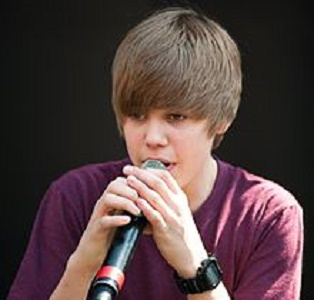
\includegraphics[width=4cm, height =6cm]{images/bieber.jpg} &
\vspace{-4cm}{Disusun oleh:\newline Nama: Edric Laksa Putra\newline NIM	: 1114065}

\end{tabular}
\end{center}
\doublespacing
{\center
\vspace{1cm}
Telah Disetujui dan Disahkan\\ Sebagai laporan Tugas Akhir Departemen Informatika\\
Institut Teknologi Harapan Bangsa\\[0.5cm]
Bandung,   Desember 2017\\
Disetujui,\\[0.5cm]
Pembimbing\\[2cm]
\bfseries 
{\underline {Irfin Afifudin, S.T., M.T.}\\
NIK. \\}}